\documentclass[../main/Notes.tex]{subfiles}
\begin{document}

\section[Signal Detection Theory III]{Signal Detection Theory III \iftoggle{showdates}{\small{\textit{2014-06-20}}}{}}

\subsection{From YN to 2AFC}\index{YN-Task}\index{2AFC}
In comparison to simple Yes-No-task there exists an alternative task design which is the 2-Alternative-Forced-Choice-task. In each trial the subject is presented with two intervals with a light stimulus in one of it, therefore there are two ``stimulations'' $X_{1}$ and $X_{2}$. The subject is then forced to state in which interval the stimulus appeared. By this we get a probability distribution for the stimulation in each interval. The probabilities for this experiment are given in the following.

\begin{align*}
\left(X_{1}|S=1\right)&\sim N\left(\Delta\mu,\sigma^{2}\right)\\
\left(X_{2}|S=1\right)&\sim N\left(0,\sigma^{2}\right)\\
\left(X_{1}|S=2\right)&\sim N\left(0,\sigma^{2}\right)\\
\left(X_{2}|S=2\right)&\sim N\left(\Delta\mu,\sigma^{2}\right)
\end{align*}

We are using again the same Gaussian's with different means. This is also referred to as \textit{equal variance signal detection model} and may be plotted like this:

\begin{figure}[ht]
\centering
\begin{tikzpicture}[scale=0.7]
  \begin{axis}[every axis plot post/.append style={mark=none, domain=-4:4, samples=50, smooth}, axis x line*=bottom, axis y line*=left, ticks=none, ylabel={S=1}, enlargelimits=upper, name=gauss]
    \addplot [red, ultra thick]    {gauss(-2,0.5)};
    \addplot [green, ultra thick]  {gauss(2.5,0.5)};
    \node [above] at (axis cs: -2, 0)  {$0$};
    \node [above] at (axis cs: 2.5, 0) {$\Delta \mu$};
  \end{axis}
  \draw [black,decorate,decoration={brace,amplitude=5pt,mirror},xshift=0.4pt,yshift=-0.4pt](0,0)   -- (3,0)   node[black,midway,yshift=-0.6cm] {\footnotesize $2^{nd}interval$};
  \draw [black,decorate,decoration={brace,amplitude=5pt,mirror},xshift=0.4pt,yshift=-0.4pt](3.5,0) -- (6.5,0) node[black,midway,yshift=-0.6cm] {\footnotesize $1^{st}interval$}; 
\end{tikzpicture}
\begin{tikzpicture}[scale=0.7]
  \begin{axis}[every axis plot post/.append style={mark=none, domain=-4:4, samples=50, smooth}, axis x line*=bottom, axis y line*=left, ticks=none, ylabel={S=2}, enlargelimits=upper, name=gauss]
    \addplot [red, ultra thick]   {gauss(-2,0.5)};
    \addplot [green, ultra thick] {gauss(2.5,0.5)};
    \node [above] at (axis cs: -2, 0)   {$0$};
    \node [above] at (axis cs:  2.5, 0) {$\Delta \mu$};
  \end{axis}
  \draw [black,decorate,decoration={brace,amplitude=5pt,mirror},xshift=0.4pt,yshift=-0.4pt](0,0)   -- (3,0)   node[black,midway,yshift=-0.6cm] {\footnotesize $1^{st}interval$};
  \draw [black,decorate,decoration={brace,amplitude=5pt,mirror},xshift=0.4pt,yshift=-0.4pt](3.5,0) -- (6.5,0) node[black,midway,yshift=-0.6cm] {\footnotesize $2^{nd}interval$};
\end{tikzpicture}
\end{figure}
If the stimulus was presented in the $1^{st}$ interval $X_2$ (our sensation for the $2^{nd}$ interval) is so to say the noise distribution and the other way around if the stimulus is shown in the $2^{nd}$ interval. If we now choose the variables $X_1$ and $X_2$ as the axis we get the following plot:

%crazy table
%\begin{tabularx}{\textwidth}{lXl}
%$\left(X_{1}|S=1\right)\sim N\left(\Delta\mu,\sigma^{2}\right)$ & {\small - The probability distribution for a stimulation in the first interval given that the signal was in the first interval} & \multirow{2}{*}{
%\begin{tikzpicture}
  %\draw[thick,decorate,decoration={brace,amplitude=3pt}] (0,2.5) -- (0,1) node[midway, right=4pt, align=left] {\small equal variance signal\\\small detection model};
%\end{tikzpicture}
%} \\
%$\left(X_{2}|S=1\right)\sim N\left(0,\sigma^{2}\right)$ & \multirow{3}{*}{  
%\begin{tikzpicture}[scale=0.5]
  %\begin{axis}[every axis plot post/.append style={mark=none, domain=-4:4, samples=50, smooth}, axis x line*=bottom, axis y line*=left, ticks=none, ylabel={S=1}, enlargelimits=upper, name=gauss]
    %\addplot [red, ultra thick]    {gauss(-2,0.5)};
    %\addplot [green, ultra thick]  {gauss(2.5,0.5)};
    %\node [above] at (axis cs: -2, 0)  {$0$};
    %\node [above] at (axis cs: 2.5, 0) {$\Delta \mu$};
  %\end{axis}
  %\draw [black,decorate,decoration={brace,amplitude=5pt,mirror},xshift=0.4pt,yshift=-0.4pt](0,0)   -- (3,0)   node[black,midway,yshift=-0.6cm] {\footnotesize $2^{nd}interval$};
  %\draw [black,decorate,decoration={brace,amplitude=5pt,mirror},xshift=0.4pt,yshift=-0.4pt](3.5,0) -- (6.5,0) node[black,midway,yshift=-0.6cm] {\footnotesize $1^{st}interval$}; 
%\end{tikzpicture}
%\begin{tikzpicture}[scale=0.5]
  %\begin{axis}[every axis plot post/.append style={mark=none, domain=-4:4, samples=50, smooth}, axis x line*=bottom, axis y line*=left, ticks=none, ylabel={S=2}, enlargelimits=upper, name=gauss]
    %\addplot [red, ultra thick]   {gauss(-2,0.5)};
    %\addplot [green, ultra thick] {gauss(2.5,0.5)};
    %\node [above] at (axis cs: -2, 0)   {$0$};
    %\node [above] at (axis cs:  2.5, 0) {$\Delta \mu$};
  %\end{axis}
  %\draw [black,decorate,decoration={brace,amplitude=5pt,mirror},xshift=0.4pt,yshift=-0.4pt](0,0)   -- (3,0)   node[black,midway,yshift=-0.6cm] {\footnotesize $1^{st}interval$};
  %\draw [black,decorate,decoration={brace,amplitude=5pt,mirror},xshift=0.4pt,yshift=-0.4pt](3.5,0) -- (6.5,0) node[black,midway,yshift=-0.6cm] {\footnotesize $2^{nd}interval$};
%\end{tikzpicture}
%} & \\
%$\left(X_{1}|S=2\right)\sim N\left(0,\sigma^{2}\right)$ & & \\
%$\left(X_{2}|S=2\right)\sim N\left(\Delta\mu,\sigma^{2}\right)$ & &
%\end{tabularx}


\begin{figure}[ht!]
\centering
\begin{tikzpicture}[scale=1]

\draw (4.7,1) circle (1cm);
\draw (4.7,1) circle (0.8cm);
\draw (4.7,1) circle (0.6cm);
\draw (4.7,1) circle (0.4cm);
\draw (4.7,1) circle (0.2cm);
\draw (1,4.7) circle (1cm);
\draw (1,4.7) circle (0.8cm);
\draw (1,4.7) circle (0.6cm);
\draw (1,4.7) circle (0.4cm);
\draw (1,4.7) circle (0.2cm);
\node [left] at (1, 3) {$X_{2}$};
\node [above] at (3, 0.5) {$X_{1}$};
\node [above] at (4.7, 2) {S=1};
\node [right] at (2 ,4.7) {S=2};
\node [left] at (5.25, 5.25) {\footnotesize decision boundary};
\draw[->, thick] (0, 1) -- (6, 1);
\draw[->, thick] (1, 0) -- (1, 6);
\draw (1, 4.7) -- (2,5.7);
\draw (4.7, 1) -- (5.7,2);

\begin{axis}[hide axis, yshift=0cm, every axis plot post/.append style={mark=none, domain=-4:5.75, samples=50, smooth}, 
    axis x line*=bottom, axis y line*=left, ticks=none, enlargelimits=upper,rotate=315, x=0.75cm, y=1.25cm]
\addplot [yellow, fill=yellow, fill opacity=0.4]  {gauss(-2.14,0.5)};
\end{axis}

\begin{axis}[hide axis,xshift=0.5cm,yshift=-0.5cm, every axis plot post/.append style={mark=none, domain=-5.5:4.25, samples=50, smooth},
    axis x line*=bottom, axis y line*=left, ticks=none, enlargelimits=upper,rotate=315, x=0.75cm, y=1.25cm ] %ticks=none,  
\addplot [yellow, fill=yellow, fill opacity=0.4]  {gauss(2.425,0.5)};
\end{axis}

\draw [fill=yellow , fill opacity=0.2] (4.7,1) -- (1,4.7) -- (1,1) circle;
\draw (1,1) -- (5.25,5.25);
\end{tikzpicture}
\end{figure}
If we could discriminate perfectly our data points would lie on the $x$ or $y$ axis for each trial (depending on the interval). When we discussed why HT-Theory is wrong (\ref{subsubsec:RelYN2AFC}), we already stated that subjects perform better in 2AFC than in YN-Tasks. Now we see why: the distance of the two distributions is $\Delta \mu_{2AFC} = \sqrt{2}\Delta\mu$. This is $>\Delta\mu$! The strategy for the best performance in 2AFC is the following:

\begin{itemize}
\item Say 1 if $X_{1} > X_{2}$
\item Say 2 if $X_{2} \geq X_{1}$
\end{itemize}

%we should maybe add here something why this is so also intuitively

We see that $\Delta X= X_{2}-X_{1} \stackrel{!}{>}0$. What is now the distribution of $\Delta X$? Note that if you scale or add normal distributions you always get again a normal distribution with scaled standard deviations and means and added variances and means.

\begin{align*}
\left(\Delta X | S = 1\right) &\sim N\left(0, \sigma^{2}\right) - N\left( \Delta \mu , 2\sigma^{2}\right) = N\left( -\Delta \mu , 2\sigma^{2}\right)\\
\left(\Delta X | S = 2\right) &\sim N\left(\Delta \mu, \sigma^{2}\right) - N\left(0, 2\sigma^{2}\right) = N \left( \Delta \mu , 2\sigma^{2}\right)
\end{align*}
We may now calculate the Signal to Noise Ratio of this two distributions.

\begin{center}
\begin{minipage}[b][3cm][t]{3.5cm}
\begin{tikzpicture}[scale=0.5]
\begin{axis}[every axis plot post/.append style={mark=none, domain=-4:4, samples=50, smooth}, 
    axis x line*=bottom, axis y line*=left, ticks=none, enlargelimits=upper, name=gauss]
    \addplot [red, ultra thick]    {gauss(-2,0.5)};% node[pos=0.4,  anchor=east] {$\sigma=0.5$};
    \addplot [green, ultra thick]  {gauss(2.5,0.5)};%   node[pos=0.6,  anchor=west] {$\sigma=1$};
    \node [above] at (axis cs:  -2, 0) {$-\Delta\mu$};
    \node [above] at (axis cs:  2.5, 0) {$\Delta \mu$};
    \node [above] at (axis cs:  -2, 0.8) {S=1};
     \node [above] at (axis cs:  2.5, 0.8) {S=2};
\end{axis}
\end{tikzpicture} 
\end{minipage}
\begin{minipage}[b][3.5cm][t]{12cm}
\begin{align*}
SNR &= \frac{\Delta\mu - (-\Delta\mu)}{\sqrt{2\sigma^2}}\\
    &= \frac{2\Delta\mu}{\sqrt{2}\sigma}\\
    &= \sqrt{2}\Delta\mu ~~~\left(\text{same result as in the geometric solution}\right)
\end{align*}
\end{minipage}
\end{center}

\subsection{Cue Combination - Ernst \& Banks (2002) - Visuo-haptic cue combination}
The task in this experiment is to judge the size of a bar when you can see and feel it. Your two measurements of s may be defined as the following:

\begin{align*}
V &\sim N\left(s,\sigma_{V}^{2}\right)\\
H &\sim N\left(s,\sigma_{H}^{2}\right)
\end{align*}

In this is example it is not wise to choose the same distribution for both measurements, since we would expect that our visual system is more accurate than the haptic one (imagine $s=2cm$).
\begin{figure}[ht!]
\centering
\begin{tikzpicture}
\begin{axis}[axis x line*=bottom, axis y line*=left, enlargelimits=upper, axis on top, domain=0:4, legend style={at={(1.2,0.8)}, anchor=east}]
    \addplot [red, ultra thick,smooth]    {gauss(2,0.8)};
    \addlegendentry{Haptics}
    \addplot [green, ultra thick,smooth]  {gauss(2,0.5)};
    \addlegendentry{Vision}
\end{axis}
\end{tikzpicture} 
\end{figure}
\newpage

Different than in the 2AFC the two distributions have the same mean- leading to the following plot: 
\begin{figure}[ht!]
\centering
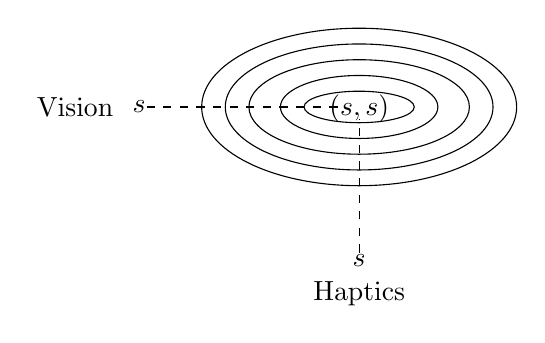
\begin{tikzpicture}
\draw (3,2.15) ellipse (2cm and 1cm);
\draw (3,2.15) ellipse (1.7cm and 0.8cm);
\draw (3,2.15) ellipse (1.4cm and 0.6cm);
\draw (3,2.15) ellipse (1cm and 0.4cm);
\draw (3,2.15) ellipse (0.7cm and 0.2cm);
\node [above] at (3, 1.825) {$(s,s)$};
\node [right] at (0, 2.15) {$s$};
\node [left] at (0, 2.15) {Vision};
\node [above] at (3, 0) {$s$};
\node [above] at (3, -0.5) {Haptics};
\draw [dashed] (0.3, 2.15) -- (2.8, 2.15);
\draw [dashed] (3, 0.3) -- (3, 2);
\end{tikzpicture}
\end{figure}

Given the length of the bar ($s$) this is the probability for our haptic ($h$) and visual ($v$) impression:
\smallskip
\begin{align*}
p\left(V=v;H=h|s\right)=\frac{1}{\sqrt{2\pi}\sigma_{V}}e^{-\frac{1}{2}\left(\frac{v-s}{\sigma_{V}}\right)^{2}}\frac{1}{\sqrt{2\pi}\sigma_{H}}e^{-\frac{1}{2}\left(\frac{h-s}{\sigma_{H}}\right)^{2}}
\end{align*}

Together with the log-likelihood we can calculate a ML-Estimate $\hat{s}$ for $s$:
\begin{align*}
\Rightarrow -\frac{1}{2}\left(\left(\frac{v-\hat{s}}{\sigma_{V}}\right)^{2} + \left(\frac{h-\hat{s}}{\sigma_{H}}\right)^{2}\right) = -\frac{1}{2}\left(\frac{v-\hat{s}}{\sigma_{V}}\right)^{2} -\frac{1}{2} \left(\frac{h-\hat{s}}{\sigma_{H}}\right)^{2}
\end{align*}
Use first derivative:

\begin{align*}
& & \left(\frac{v-\hat{s}}{\sigma_{V}}\right) \frac{2}{2\sigma_{V}} + \left(\frac{h-\hat{s}}{\sigma_{H}}\right) \frac{2}{2\sigma_{H}} & \stackrel{!}{=}0 & & \\
\Leftrightarrow & & \frac{v-\hat{s}}{\sigma_{V}^{2}} + \frac{h-\hat{s}}{\sigma_{H}^{2}} & = 0 & & \\
\Leftrightarrow & & \frac{v}{\sigma_{V}^{2}} + \frac{h}{\sigma_{H}^{2}} -\hat{s} \left(\frac{1}{\sigma_{V}^{2}} + \frac{1}{\sigma_{H}^{2}}\right) & = 0 & & \\
\Leftrightarrow & & \frac{v}{\sigma_{V}^{2}} + \frac{h}{\sigma_{H}^{2}} & = \hat{s} \left(\frac{1}{\sigma_{V}^{2}} + \frac{1}{\sigma_{H}^{2}}\right) & & \\
\Leftrightarrow & & \hat{s} & = \left(\frac{v}{\sigma_{V}^{2}} + \frac{h}{\sigma_{H}^{2}}\right) \frac{\sigma_{V}^{2}\sigma_{H}^{2}}{\sigma_{V}^{2} + \sigma_{H}^{2}} & & \\
\Leftrightarrow & & \hat{s} & = \frac{v\sigma_{H}^{2}}{\sigma_{V}^{2} + \sigma_{H}^{2}} + \frac{h\sigma_{V}^{2}}{\sigma_{V}^{2} + \sigma_{H}^{2}} & &
\end{align*}

This estimate seems logical, since the variances are used as a normalization term in the denominator and the numerator weights our sensation according to their internal variance. In our example we assumed the visual system to have a small variance compared to the haptic system, so the $v$ has greater impact on $\hat{s}$.

\end{document}

